\chapter{Panorama Econômico}
\par A eclosão da pandemia do coronavírus tem se mostrado o maior choque enfrentado pela economia brasileira, tanto pela demanda com a contração do consumo das famílias e dos investimentos, quanto pelo lado da oferta, com empresas indo à falência. A fragilidade fiscal do Estado brasileiro e a alta taxa de desemprego desde a recessão de 2015/2016 ajudam a compor um cenário bastante desafiador para as economias do Brasil e do Tocantins.
%\par Nesse sentido, espera-se também um grande choque na economia tocantinense. Os indicadores que serão apresentados ao longo das seções deste Boletim farão um retrato de como esse grande choque afetou e poderá afetar a economia do nosso estado.
\begin{figure}[!h]
	\begin{subfigure}{\linewidth}
		\caption{Expectativa de crescimento anual do PIB Nacional}
		\subcap{Média por setor}
		\label{fig:expectativa_pib}
		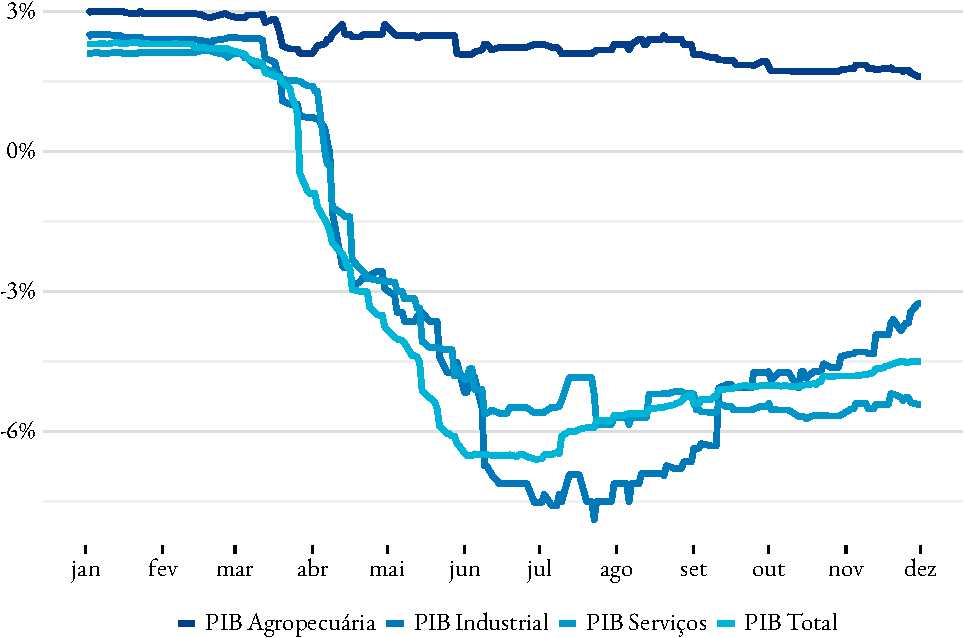
\includegraphics{fig/pib_expec-1.pdf}
		\source{\abbr{bcb}}
	\end{subfigure}
	\begin{subfigure}{\linewidth}
		\caption{Variação trimestral do PIB pelo lado da demanda}
		\subcap{Com ajuste sazonal}
		\label{fig:pib_demanda}
		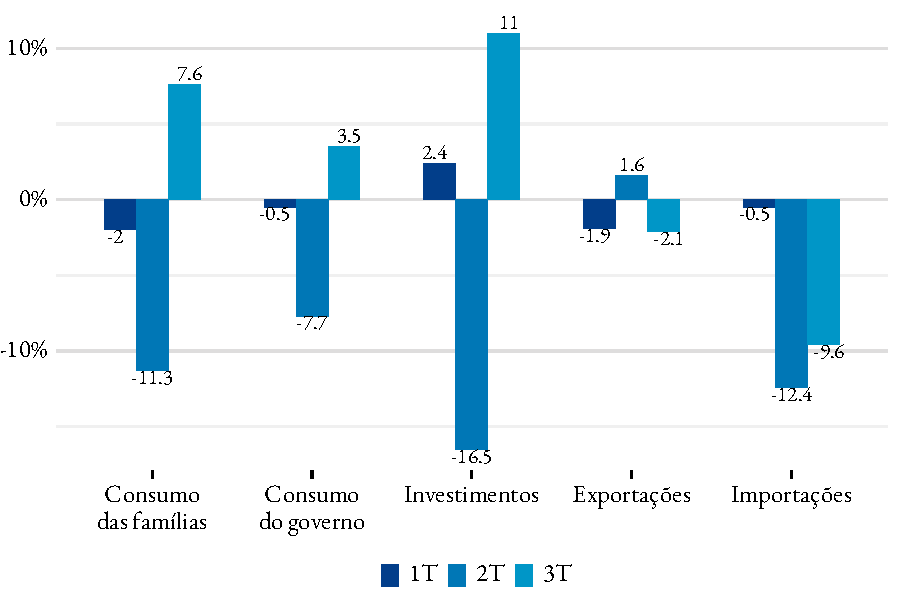
\includegraphics{fig/pib_demanda.pdf}
		\source{\abbr{ibge}}
		\notes{\trimestres[1-3]}
	\end{subfigure}
	\begin{subfigure}{\linewidth}
		\caption{Variação trimestral do PIB pelo lado da oferta}
		\subcap{Com ajuste sazonal}
		\label{fig:pib_oferta}
		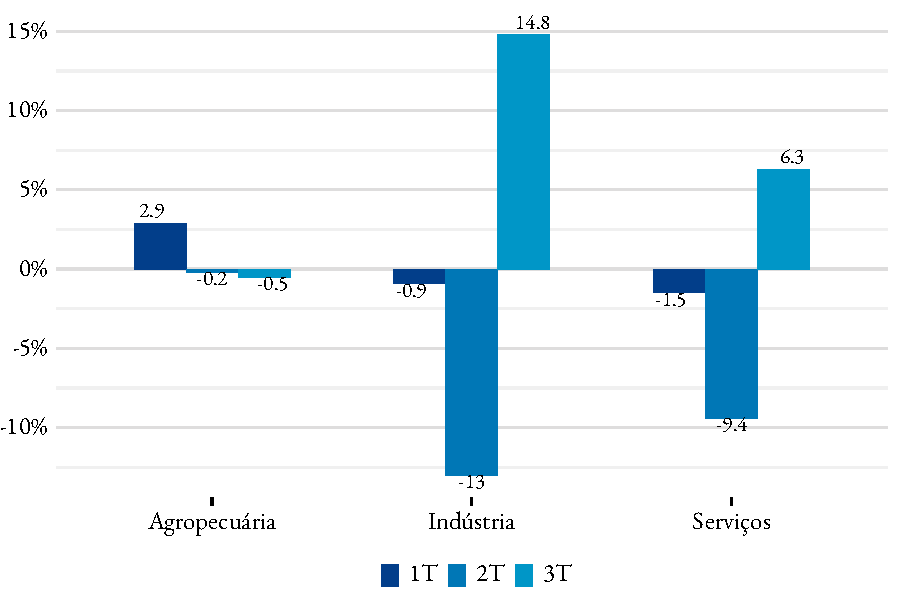
\includegraphics{fig/pib_oferta.pdf}
		\source{\abbr{ibge}}
		\notes{\trimestres[1-3]}
	\end{subfigure}
\end{figure}
\par As expectativas de crescimento para a economia brasileira situavam-se em torno de 2,3\% ainda no início do ano como mostra a \ref{fig:expectativa_pib}. As taxas esperadas para indústria e serviços seguiam próximas ao valor esperado para o \abbr{pib}. Já para o setor agropecuário a expectativa de crescimento era um pouco mais otimista, com uma variação esperada por volta de 3\%. Durante praticamento todo primeiro trimestre as expectativas mantiveram-se estáveis até o início da pandemia em meados de março.
\par As expectativas de crescimento começam a cair a partir da propagação da covid-19 por todo o mundo. Já em abril as projeções de crescimento esperavam uma queda do \abbr{pib} para o ano de 2020, tornando-se cada vez mais pessimistas nos meses decorrentes. O período de maior pessimismo foi no meio do ano, onde se esperava uma contração maior que 6\% para o ano.
%\par Já no primeiro trimestre a economia brasileira encolheu 1.5\% de acordo com dados oficiais do IBGE. Pelo lado da demanda, como é mostrado na \ref{fig:pib_demanda}, a maior contração foi no consumo das famílias e nas exportações, com quedas de -2\% e -1,9\%, respectivamente. Investimento foi o único que apresentou um crescimento de 2,4\%. Cabe destacar que a pandemia só inicia no fim do trimestre, o que pode indicar que já havia uma perca de dinamismo da atividade econômica antes mesmo da chegada do vírus, dado a magnitude da contração observada.
\par No primeiro trimestre de 2020 o \abbr{pib} brasileiro encolheu 1,5\% de acordo com dados oficiais do \abbr{ibge}. Cabe destacar que a pandemia só inicia no fim do trimestre, o que pode indicar que já havia uma perca de dinamismo da atividade econômica antes mesmo da chegada do vírus, dado a magnitude da contração observada. O segundo trimestre foi o de maior contração, com uma queda de 9,6\%, muito em função dos maiores esforços de isolamento social feitos nesse período. No terceiro trimestre, houve um crescimento de 7,7\%, que apesar de alto não foi suficiente para repor as perdas no início do ano.
\begin{smbox}[label={labelbox},nameref={Cálculo do PIB e as suas óticas}]{Cálculo do PIB e as suas óticas}
	O \abbr{pib} é a soma do valor de todos os bens e serviços finais produzidos por um país durante um ano. É possível calcula-lo por três óticas diferenets, pela oferta, somando tudo aquilo que é produzido por todos os setores, pela da demanda, somando o consumo das famílias, consumo do governo, investimentos e exportações liquidas (exportações menos importações) e também pela ótica da renda, somando toda renda da população. O resultado das três óticas é sempre o mesmo.
\end{smbox}
\par No lado da demanda conforme a Figura \ref{fig:pib_demanda} é possível ver que todos os componentes em algum dos períodos analisados registraram queda. Como já foi abordado, o segundo semestre foi o que apresentou os piores resultados, com apenas as exportações registrando uma alta de 1,6\% . No movimento de retomada do terceiro trimestre é possível observar que grande parte do aumento de 7,7\% é explicado pela retomada do consumo das famílias e investimentos, tendo em vista o tamanho desses componentes no \abbr{pib} total e as altas taxas de crescimento.
\par Pelo lado da oferta apresentado na Figura \ref{fig:pib_oferta} o único setor com resultados mais estáveis foi o agropecuário, setor menos afetado pelos esforços de isolamento, e o que em parte explica o bom desempenho das exportações no lado da demanda. No setor de serviços, que representa mais que 70\% do \abbr{pib}, as quedas de 1.5\% e 9,4\% nos dois primeiros trimestres pesaram bastante. Já as quedas de 0,9\% e 13\% da indústria demonstram a fragilidade desse setor dentro da economia brasileira.
%\par No quarto trimestre as expectativas do PIB total apresentou um leve crescimento, as últimas projeções de 2020 apontam contração de -4,36\%. Já a mediana das expectativas do PIB da industria mostrou uma leve recuperação nos útimos três meses, finalizando o ano com -3,9\%. Serviçõs também exibiu uma tímida recuperação, finalizando com -4,8\%. O setor agropecuário, menos afetado, ao longo de todo o ano teve expectativa de crescimento acima de 1,5\%, teve reduções ao longo de 2020, mas finalizou o ano com projeção de crescimento de 2,32\%.
\par Um ponto a ser colocado é que os dados oficias do \abbr{pib} de 2020 para estados ainda não foram divulgados pelo \abbr{ibge}, o que não nos permite fazer uma análise mais profunda sobre o desempenho da economia tocantinense no período. Assim, a análise dos dados da Pesquisa Mensal do Comércio (\abbr{pmc}) pode ser útil para se ter uma noção de como a economia do estado performou ao longo do ano. Para isso apresenta-se na Figura \ref{fig:pmc} os dados de variação mensal do volume de vendas do comércio para o Brasil e para o Tocantins.

\begin{smbox}[label={labelbox},nameref={Pesquisa Mensal do Comércio(PMC)}]{Pesquisa Mensal do Comércio (PMC)}
A \abbr{pmc} produz indicadores que permitem acompanhar o comportamento conjuntural do comércio varejista no país, investigando a receita bruta de revenda nas empresas formalmente constituídas, com 20 ou mais pessoas ocupadas, e cuja atividade principal é o comércio varejista.
\end{smbox}

\par O período de março a abril foram os meses em que houveram maiores contrações no volume de serviços, conforme a Figura \ref{fig:pms} tanto para o Tocantins quanto para a região Norte. Amazonas e Pará tiveram quedas superiores ao do estado tocantinense. O Tocantins teve uma queda de 3\%, nos dois estados da região norte a queda foi superior a 3,5\%. Ao final do primeiro semestre do ano vigente, o volume de serviços não conseguiu uma recuperar as suas baixas, como ocorreu no volume de vendas no comércio varejista. A queda dos serviços continua para o estado do Tocantins, chegando a ter uma queda de -6,5\%. Os estados da região norte conseguiram estabilizar essa queda, apresentando valores de -1,5\% a -2,0\%. O primeiro semestre foi impactante para os serviços, demonstrando que ainda não há uma recuperação para o índice e apresentando, números preocupantes para o estado do Tocantins.
\par O comércio varejista também sofreu no período de março a abril, na qual, os estados da região norte apresentaram quedas similares ao volume de serviços. Na Figura \ref{fig:pmc}, os estados do Amazonas e Pará apresentam quedas mais bruscas do que ao Tocantins. No Amazonas a queda foi de -4,8\% no primeiro trimestre, já o Pará apresenta uma queda similar de -4,2\%. Demonstrando que esses dois estados foram os mais atingidos pelo efeito da atual pandemia. Já o Tocantins teve uma queda menor em comparação aos dois, apresentando o valor de -0,8\%. Diferente do volume de serviços, ocorre uma recuperação nas vendas do comércio varejista, que provavelmente foi auxiliado pelos pacotes econômicos do governo federal. Os estados do Amazonas e Pará apresentaram valores positivos no índice, chegando aos resultados de 4,7\% e 5,9\%, demonstrando uma recuperação ao final do primeiro semestre. E por fim, o Tocantins apresenta um valor menor aos estados da região, com o valor de 2,7\%. Só que diferente dos dois estados, o volume de vendas para o Tocantins não chegou a apresentar resultados tão baixos ao ponto de conseguir manter bons números de vendas no comércio varejista.
%\par A atividade comercial no estado do Tocantins é de grande importância para a construção do PIB estadual. Até a atual formulação deste boletim, são apresentados dois índices que compõe a PMC, são eles: Serviços e Vendas no comércio varejista.
%\par Na Figura \ref{fig:pmc}, o setor de serviços sofrem com maiores variações. Analisando os dados a partir de março de 2019 até setembro do nosso ano de exercício, é apresentado uma recuperação desse setor até Março do ano atual. Uma justificativa para as variações negativas do setor de serviços até o atual momento, são as medidas de isolamento social para a contenção do Covid-19, assim, se encerra um período de variações positivas no setor que teve inicio em março de 2019.
%\par O comércio varejista tem uma relação evidente com o setor de serviços, entretanto, não sofreu com altas variações como o setor de serviços. Em março de 2019, o setor vinha de uma queda semelhante ao de serviços, mas, a partir desse momento obteve variações positivas até março do atual ano. A queda na variação do comércio varejista foi amenizada, mesmo no contexto da Covid-19 pelos estímulos que a economia recebeu para lidar com a atual pandemia, o que pode se justificar essa queda mais suavizada do que o setor de serviços.
\begin{figure}[!h]
	\begin{subfigure}{\linewidth}
		\caption{Variação mensal do volume de vendas no comércio varejista}
		\label{fig:pmc}
		\subcap{Variação acumulada no ano (base: igual período do ano anterior)}
		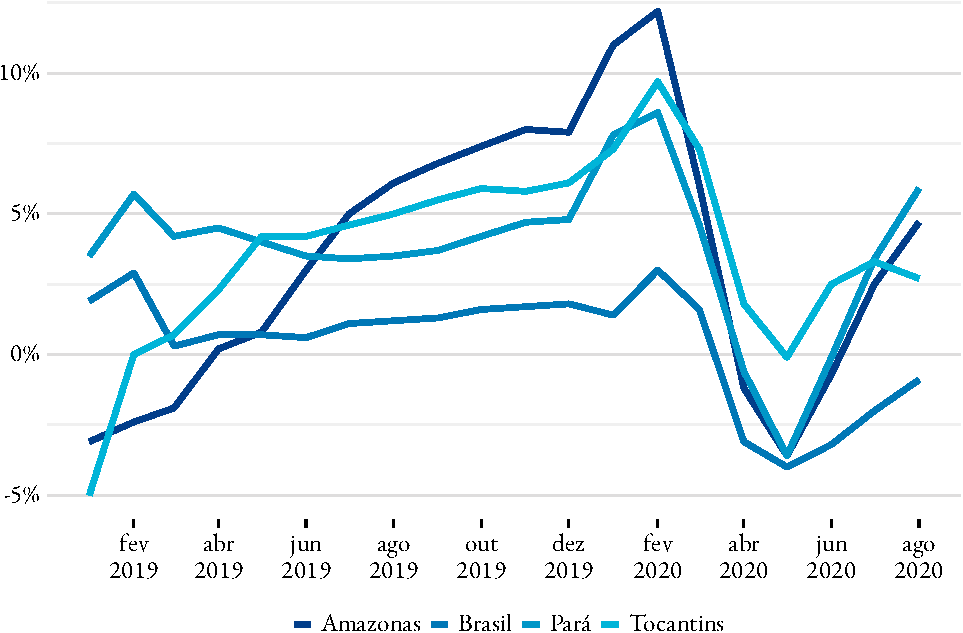
\includegraphics{fig/pmc_ibge-1.pdf}
		\source{\abbr{ibge}}
	\end{subfigure}
	\begin{subfigure}{\linewidth}
		\caption{Variação mensal do volume de serviços}
		\label{fig:pms}
		\subcap{Variação acumulada no ano (base: igual período do ano anterior)}
		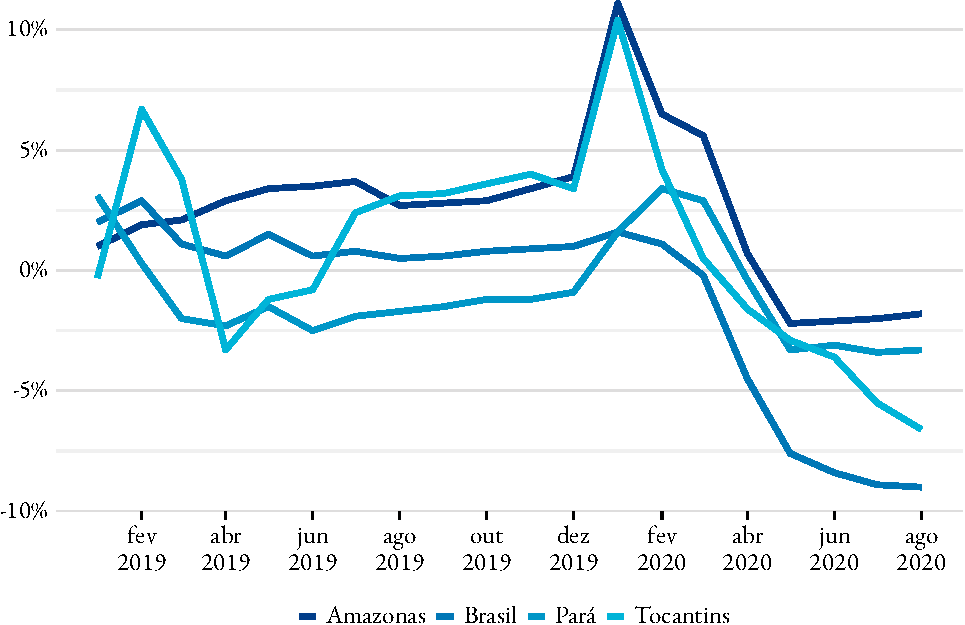
\includegraphics{fig/pms_ibge-1.pdf}
		\source{\abbr{ibge}}
	\end{subfigure}
\end{figure}